

Microcontroladores são circuitos integrados compactos desenvolvidos para governar
uma operação específica em um sistema embarcado. No contexto da aplicação deste
trabalho, o uso de um microcontrolador é fundamental para se obter o controle
desejado de trajetória e posicionamento do robô.

\subsection{STM32 - STM32F103C8}

STM32 é uma família de microcontroladores de 32-bits fabricados pela
ST-Microelectronics. O processador empregado nessa família é o ARM Cortex-M3 (\cite{cortex_m3}),
baseado em arquitetura Harvard, de 32-bits. Os microcontroladores STM32 fornecem
base para uma uma grande variedades de sistemas embarcados, com custo inferior
e maior flexibilidade quando comparado ao Arduino com ATmega, que possui
microcontroladores de 8 a 16 bits. Contudo, essa flexibilidade e baixo custo têm
como contrapartida o requerimento de um maior nível de experiência em
programação C do que o necessário para desenvolver as mesmas soluções em
Arduino (cuja concepção teve como objetivo maior acessibilidade para iniciantes
em programação em geral, e também  em desenvolvimento de aplicações com
microcontroladores.

O STM32F103C8 (abreviado como STM32 ao longo deste trabalho),
também conhecido como Blue Pill. Tem 64Kbs de memória flash.  De acordo com o \textit{livro Discovering the STM32 Microcontroller} (\cite{stm_doc}) e 
a documentação colaborativa (\cite{stm32_base_org}) do projeto STM32-base (\cite{stm32_base}),
possui também 7 timers, 2 ADCs, e 9 interfaces de comunicação, incluindo I2C (\textit{Inter-Integrated Circuit}), USART 
\textit{Universal Synchronous Asynchronous Receiver Transmitter}), SPI (\textit{Serial Peripheral Interface}), CAN e
USB 2.0. O STM32 apresenta 7 pinos que suportam canais de PWM de 5V, e outros 8 canais de 3.3V, e pode ser alimentado
via microUSB de 5V. Existem 3 grupos de pinos,  $P_{A}$,  $P_{B}$ e  $P_{C}$: os pinos PA vão de $P_{A0}$ 
a $P_{A15}$, PB indo de $P_{B0}$ a $P_{B15}$, e PC com apenas 3 pinos, $P_{C13}$, $P_{C14}$ e $P_{C15}$.
A relação geral dos pinos pode ser melhor obervada na figura \ref{stm32f103c8_pinout}.

\begin{figure}[htb]
	\centering
	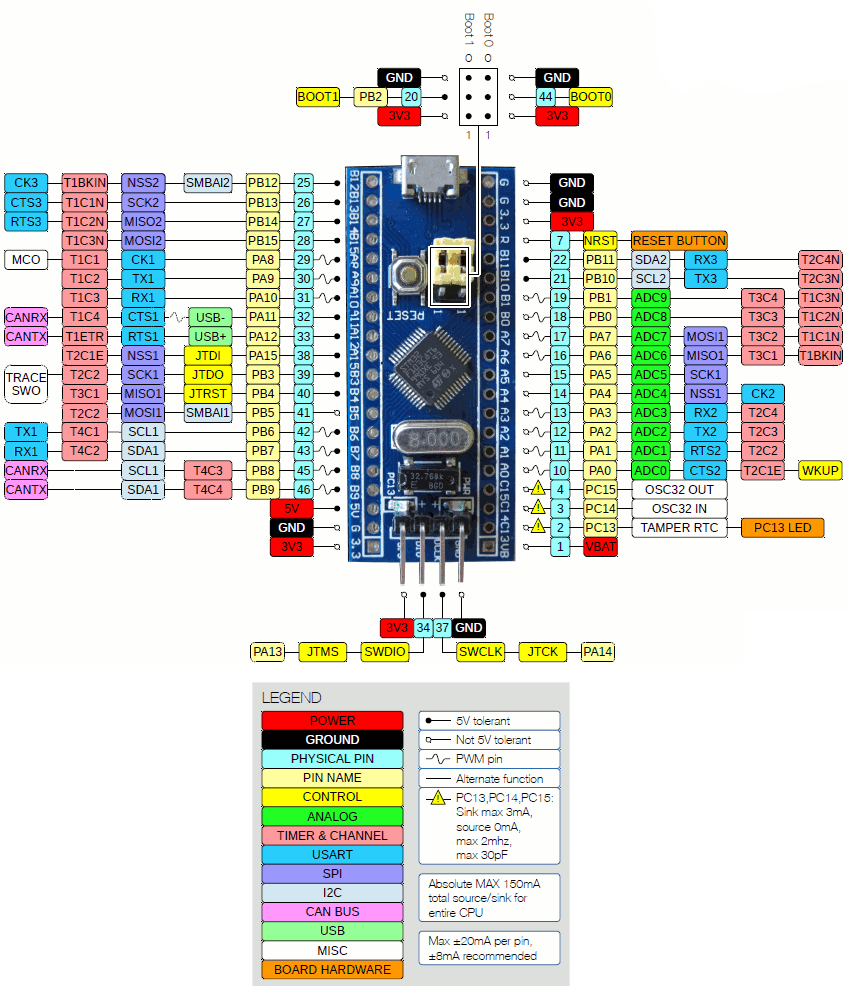
\includegraphics[width=1.0\textwidth]{figures/stm32f1_pinout}
	\caption{Diagrama de pinos do STM32F103C8}
    \label{stm32f103c8_pinout}
\end{figure}

Para carregar o projeto no microcontrolador, tem por padrão o uso do gravador ST-LINK v2.
O ST-link, cujo original (figura \ref{stlinkv2_original}) é fabricado pela ST-Microelectronics \cite{st_link_v2}, 
possui uma versão paralela mais barata
comercializada online (figura \ref{stlinkv2_cheap}), porém a versão paralelo costuma ter fabricantes diversos e 
muitas vezes não descritos na distribuição do produto 
e a relação de pinos pode variar (figura \ref{stlinkv2_cheap_pin_diff}).


\begin{figure}[htb]
	\centering
	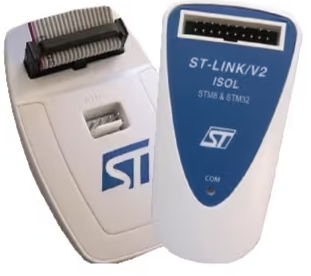
\includegraphics[width=0.5\textwidth]{figures/stlinkv2_original}
	\caption{St-Link V2 original fabricado pela ST-Microelectronics \cite{st_link_v2}}
    \label{stlinkv2_original}
\end{figure}


\begin{figure}[htb]
	\centering
	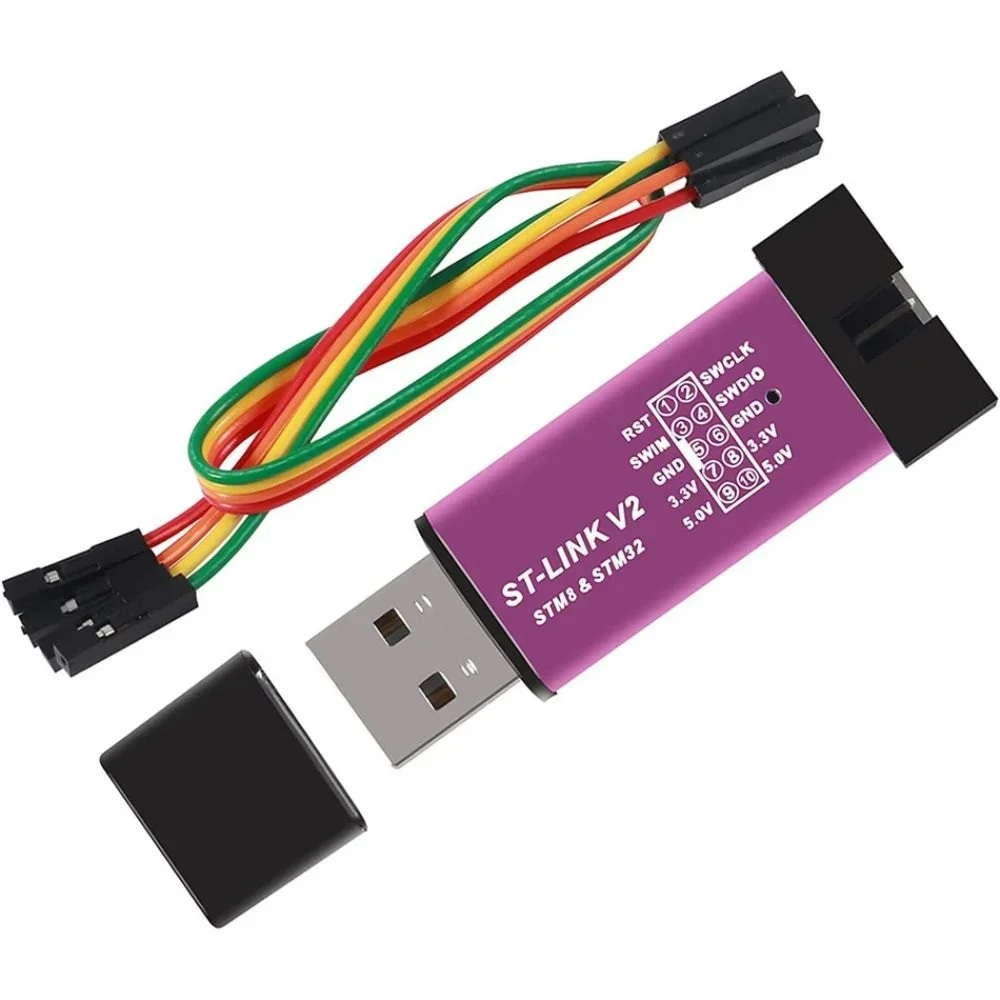
\includegraphics[width=0.5\textwidth]{figures/stlinkv2_cheap}
	\caption{St-Link V2 paralelo de fabricação desconhecida}
    \label{stlinkv2_cheap}
\end{figure}


\begin{figure}[htb]
	\centering
	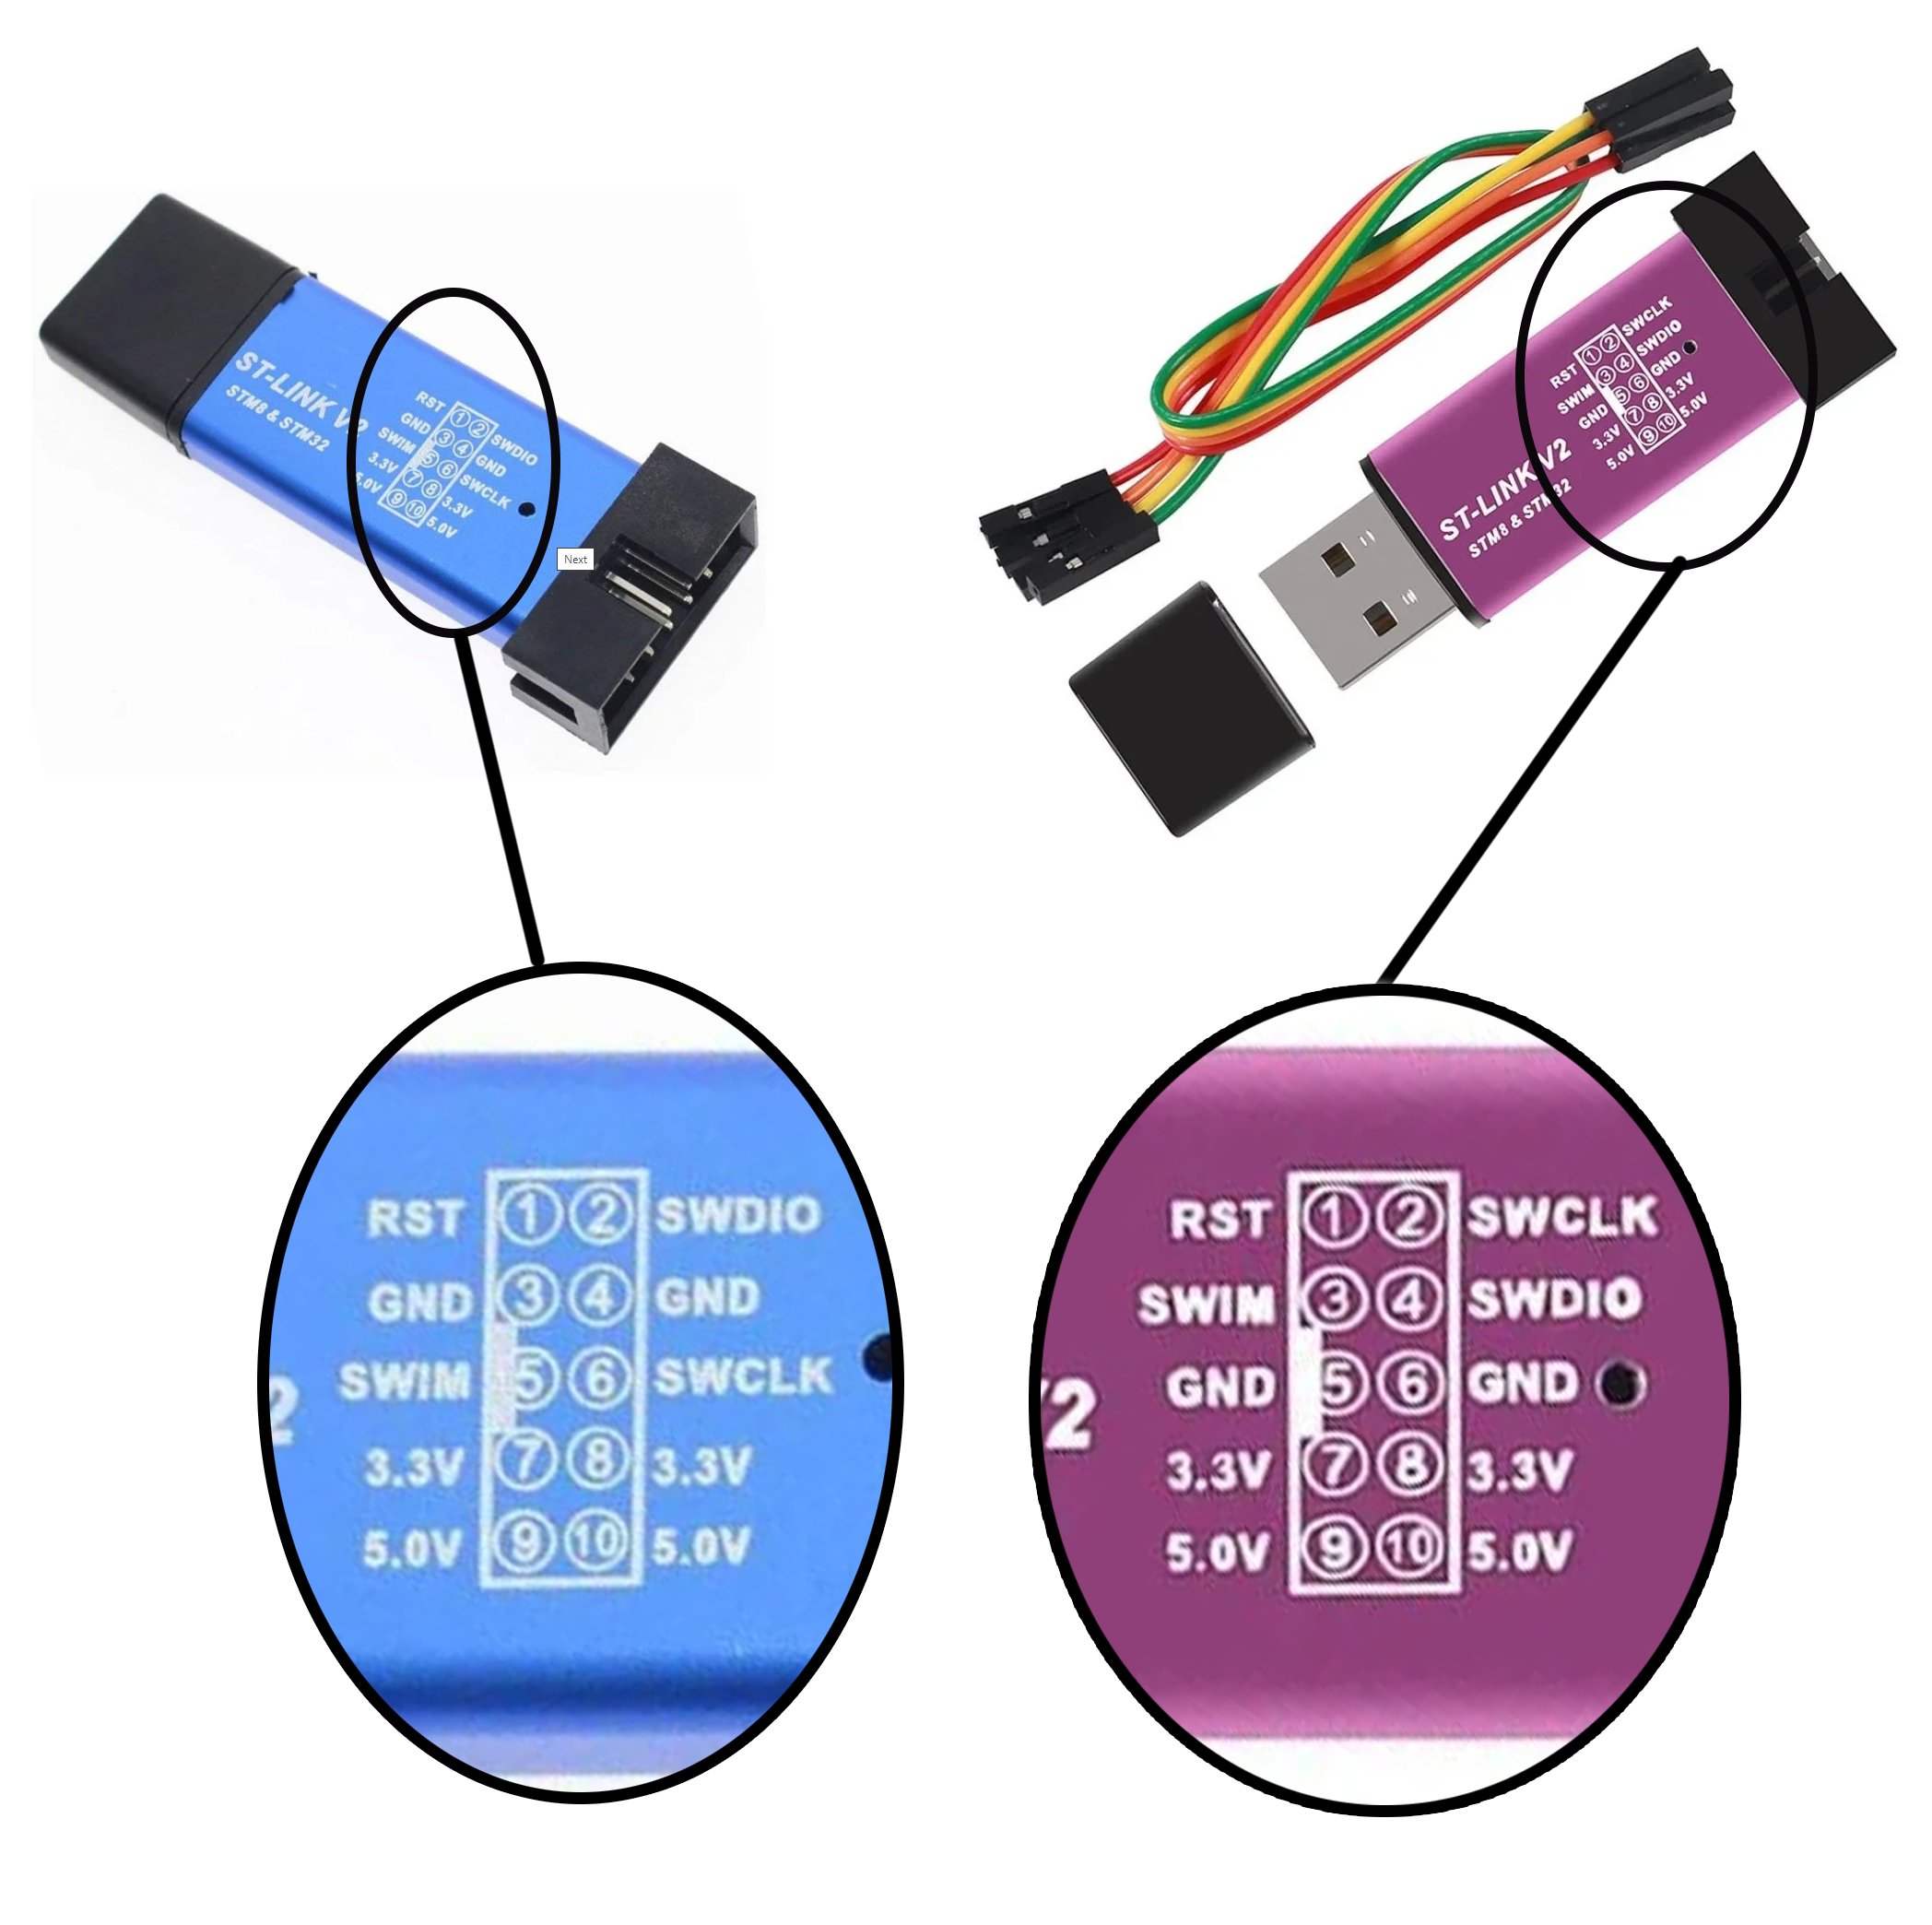
\includegraphics[width=0.5\textwidth]{figures/stlinkv2_cheap_pin_diff}
	\caption{St-Link V2 paralelo e o problema da não padronização de pinos}
    \label{stlinkv2_cheap}
\end{figure}





\subsection{ESP32 Devkit v1}




% ESP32 Series
% core = ESP32-D0WD-V3
% ESP32-WROOM-32E - https://www.espressif.com/sites/default/files/documentation/esp32-wroom-32e_esp32-wroom-32ue_datasheet_en.pdf

% https://olddocs.zerynth.com/r2.4.2/official/board.zerynth.doit_esp32/docs/index.html



